%% This template can be used to write a paper for
%% Computer Physics Communications using LaTeX.
%% For authors who want to write a computer program description,
%% an example Program Summary is included that only has to be
%% completed and which will give the correct layout in the
%% preprint and the journal.
%% The `elsarticle' style is used and more information on this style
%% can be found at
%% http://www.elsevier.com/wps/find/authorsview.authors/elsarticle.
%%
%%
\documentclass[final,3p,times]{elsarticle}

%% Use the option review to obtain double line spacing
%% \documentclass[preprint,review,12pt]{elsarticle}

%% Use the options 1p,twocolumn; 3p; 3p,twocolumn; 5p; or 5p,twocolumn
%% for a journal layout:
%% \documentclass[final,1p,times]{elsarticle}
%% \documentclass[final,1p,times,twocolumn]{elsarticle}
%% \documentclass[final,3p,times]{elsarticle}
%% \documentclass[final,3p,times,twocolumn]{elsarticle}
%% \documentclass[final,5p,times]{elsarticle}
%% \documentclass[final,5p,times,twocolumn]{elsarticle}

%% if you use PostScript figures in your article
%% use the graphics package for simple commands
%% \usepackage{graphics}
%% or use the graphicx package for more complicated commands
%% \usepackage{graphicx}
%% or use the epsfig package if you prefer to use the old commands
%% \usepackage{epsfig}

\usepackage{amssymb}
\usepackage{amsmath}
\usepackage{amsthm}
\usepackage{xcolor}
\usepackage{hyperref}
\usepackage{caption}
\usepackage{subcaption}

\hypersetup{
	unicode=true,
	pdftitle={A descriptive title},
	pdfnewwindow=true,
	colorlinks=true, 	% (false,true)
	pdfborder={0 0 0},
	linkcolor=blue,
	linktoc=all, 		% (none,all)
	citecolor=blue,
	urlcolor=blue,
	breaklinks=false,
}
%% The lineno packages adds line numbers. Start line numbering with
%% \begin{linenumbers}, end it with \end{linenumbers}. Or switch it on
%% for the whole article with \linenumbers after \end{frontmatter}.
%% \usepackage{lineno}

%% natbib.sty is loaded by default. However, natbib options can be
%% provided with \biboptions{...} command. Following options are
%% valid:

%%   round  -  round parentheses are used (default)
%%   square -  square brackets are used   [option]
%%   curly  -  curly braces are used      {option}
%%   angle  -  angle brackets are used    <option>
%%   semicolon  -  multiple citations separated by semi-colon
%%   colon  - same as semicolon, an earlier confusion
%%   comma  -  separated by comma
%%   numbers-  selects numerical citations
%%   super  -  numerical citations as superscripts
%%   sort   -  sorts multiple citations according to order in ref. list
%%   sort&compress   -  like sort, but also compresses numerical citations
%%   compress - compresses without sorting
%%
%% \biboptions{comma,round}

% \biboptions{}

%% This list environment is used for the references in the
%% Program Summary
%%
\newcounter{bla}
\newenvironment{refnummer}{%
\list{[\arabic{bla}]}%
{\usecounter{bla}%
 \setlength{\itemindent}{0pt}%
 \setlength{\topsep}{0pt}%
 \setlength{\itemsep}{0pt}%
 \setlength{\labelsep}{2pt}%
 \setlength{\listparindent}{0pt}%
 \settowidth{\labelwidth}{[9]}%
 \setlength{\leftmargin}{\labelwidth}%
 \addtolength{\leftmargin}{\labelsep}%
 \setlength{\rightmargin}{0pt}}}
 {\endlist}

\journal{Computer Physics Communications}


\newcommand\WaterLily[0]{\textsc{WaterLily}~}

\begin{document}

\begin{frontmatter}

%% Title, authors and addresses

%% use the tnoteref command within \title for footnotes;
%% use the tnotetext command for the associated footnote;
%% use the fnref command within \author or \address for footnotes;
%% use the fntext command for the associated footnote;
%% use the corref command within \author for corresponding author footnotes;
%% use the cortext command for the associated footnote;
%% use the ead command for the email address,
%% and the form \ead[url] for the home page:
%%
%% \title{Title\tnoteref{label1}}
%% \tnotetext[label1]{}
%% \author{Name\corref{cor1}\fnref{label2}}
%% \ead{email address}
%% \ead[url]{home page}
%% \fntext[label2]{}
%% \cortext[cor1]{}
%% \address{Address\fnref{label3}}
%% \fntext[label3]{}

\title{WaterLily.jl: A differentiable Julia solver to simulate incompressible fluid flow and dynamic bodies with heterogeneous execution}

%% use optional labels to link authors explicitly to addresses:
%% \author[label1,label2]{<author name>}
%% \address[label1]{<address>}
%% \address[label2]{<address>}

\author[a]{First Author\corref{author}}
\author[a,b]{Second Author}
\author[b]{Third Author}

\cortext[author] {Corresponding author.\\\textit{E-mail address:} firstAuthor@somewhere.edu}
\address[a]{First Address}
\address[b]{Second Address}

% A submitted program is expected to satisfy the following criteria: it must be of benefit to other physicists, or be an exemplar of good programming practice, or illustrate new or novel programming techniques which are of importance to computational physics community; it should be implemented in a language and executable on hardware that is widely available and well documented; it should meet accepted standards for scientific programming; it should be adequately documented and, where appropriate, supplied with a separate User Manual, which together with the manuscript should make clear the structure, functionality, installation, and operation of the program.

% Your manuscript and figure sources should be submitted through Editorial Manager (EM) by using the online submission tool at \\
% https://www.editorialmanager.com/comphy/.

% In addition to the manuscript you must supply: the program source code; a README file giving the names and a brief description of the files/directory structure that make up the package and clear instructions on the installation and execution of the program; sample input and output data for at least one comprehensive test run; and, where appropriate, a user manual.

% A compressed archive program file or files, containing these items, should be uploaded at the "Attach Files" stage of the EM submission.

% For files larger than 1Gb, if difficulties are encountered during upload the author should contact the Technical Editor at cpc.mendeley@gmail.com.

\begin{abstract}
Integrating computational fluid dynamics (CFD) software into optimization and machine-learning frameworks is hampered by the rigidity of classic computational languages and the slow performance of more flexible high-level languages.
WaterLily.jl is an open-source incompressible viscous flow solver written in the Julia language.
The small code base is multidimensional, multi-platform and backend-agnostic (serial CPU, multithreaded, \& GPU execution).
The computational time per time step scales linearly with the number of degrees of freedom on CPUs, and we see up to a 200x speed-up using CUDA kernels. This leads to comparable performance with Fortran solvers on many research-scale problems opening up exciting possible future applications on the cutting edge of machine-learning research.
% The simulator is differentiable and uses automatic-differentiation internally to immerse solid geometries and optimize the pressure solver.
\end{abstract}

\begin{keyword}
heterogeneous programming; Cartesian-grid methods; Julia; GPU
\end{keyword}

\end{frontmatter}

%%
%% Start line numbering here if you want
%%
% \linenumbers

% All CPiP articles must contain the following
% PROGRAM SUMMARY.

% {\bf PROGRAM SUMMARY/NEW VERSION PROGRAM SUMMARY}
  %Delete as appropriate.
{\bf PROGRAM SUMMARY}
\\
\\
\begin{small}
\noindent
{\em Program Title:} WaterLily.jl \\
{\em CPC Library link to program files:} (to be added by Technical Editor) \\
{\em Developer's repository link:} https://github.com/weymouth/WaterLily.jl \\
{\em Code Ocean capsule:} (to be added by Technical Editor)\\
{\em Licensing provisions(please choose one):} MIT \\
{\em Programming language:} Julia \\
{\em Supplementary material:} \\
  % Fill in if necessary, otherwise leave out.
% {\em Journal reference of previous version:}*                  \\
  %Only required for a New Version summary, otherwise leave out.
% {\em Does the new version supersede the previous version?:}*   \\
  %Only required for a New Version summary, otherwise leave out.
% {\em Reasons for the new version:*}\\
  %Only required for a New Version summary, otherwise leave out.
% {\em Summary of revisions:}*\\
  %Only required for a New Version summary, otherwise leave out.
{\em Nature of problem(approx. 50-250 words):}\\
  %Describe the nature of the problem here. \\
{\em Solution method(approx. 50-250 words):}\\
  %Describe the method solution here.
{\em Additional comments including restrictions and unusual features (approx. 50-250 words):}\\
  %Provide any additional comments here.

\begin{thebibliography}{0}
\bibitem{1}Program summary reference 1         % This list should only contain those items referenced in the
\bibitem{2}Program summary reference 2         % Program Summary section.
\bibitem{3}Program summary reference 3         % Type references in text as [1], [2], etc.
                               % This list is different from the bibliography at the end of
                               % the Long Write-Up.
\end{thebibliography}
% * Items marked with an asterisk are only required for new versions
% of programs previously published in the CPC Program Library.\\
\end{small}


\section{Introduction}

During the last decade, the computational fluid dynamics (CFD) community has embraced the surge of machine learning (ML) and the new developments in hardware architecture, such as general-purpose GPUs. Hence, classic CFD solvers based on low-level programming languages (C, Fortran) and CPU memory-distributed execution are now adapted to accommodate these new tools. On one hand, the integration of high-level ML libraries and low-level CFD solvers is not straight-forward, aka. the two-language problem \cite{Churavy2022}. When deploying a ML model online with the CFD solver, data exchange is often performed at disk level, significantly slowing down the overall runtime because of disk read/write operations. An improved way to exchange data is performed through memory, either using Unix sockets \cite{Rabault2019, Font2021}, message-passing interface (MPI) \cite{Guastoni2023}, or an in-memory distributed database \cite{Kurz2022,Font2024}, which increases the software complexity. On the other hand, porting classic CFD solvers to GPU is also a non-trivial task which often requires the input and expertise of GPU vendors \cite{Romero2022}. Still, the CFD community has been an active asset in this transition, and it currently offers a rich variety of open-source multi-GPU solvers as summarised in table \ref{tab:solvers}.

\begin{table}[!ht]
\hspace{-1.5cm}
\begin{tabular}{ l  l  l  l}
    \hline
    \multicolumn{1}{l}{\textbf{Name}} & \multicolumn{1}{l}{\textbf{Application}} & \multicolumn{1}{l}{\textbf{Method}} & \multicolumn{1}{l}{\textbf{Language}} \\
    \hline\hline
    CANS \cite{Costa2018} & Incompressible canonical flows on Cartesian grids & FDM & Fortran/OpenACC \\
    GAL{\AE}XI \cite{Kempf2024} & Compressible flows on unstructured grids & DG & CUDA-Fortran \\
    nekRS \cite{Fischer2022} & Incompressible flows on unstructured grids & SEM & C++/OCCA \\
    OpenSBLI \cite{Lusher2021} & Code-generation system for compressible flows on structured grids & FDM & Python + CUDA/OpenCL \\
    PyFR \cite{Witherden2015} & Compressible flows on unstructured grids & FR & Python + C/OpenMP, CUDA, OpenCL \\
    RHEA \cite{Jofre2023} & Compressible flows on Cartesian grids & FDM & C++/OpenACC \\
    SOD2D \cite{Gasparino2024} & Compressible/incompressible flows on unstructured grids & SEM & Fortran/OpenACC \\
    STREAmS \cite{Bernardini2021} & Compressible canonical wall-bounded flows on Cartesian grids & FDM & CUDA-Fortran \\
    \hline
\end{tabular}
\caption{Examples of multi-GPU open-source CFD solvers. Methods are abbreviated as: finite difference method (FEM), discontinous Galerkin (DG), spectral element method (SEM), and flux reconstruction (FR).}\label{tab:solvers}
\end{table}

In this context, Julia \cite{Bezanson2017} emerges as an open-source, compiled, dynamic, and composable programming language specifically designed for scientific computing which can help tackle such software challenges. High-level libraries and low level code can co-exist without compromising computing performance. Moreover, its excellent meta-programming capabilities, dynamic types, and multiple-dispatch strategy maximizes code re-usability. A great example of this is the KernelAbstractions.jl library \cite{Churavy2023}, which enables writing heterogeneous kernels for different backends (multi-threaded CPU, NVIDIA, AMD, and others) in a single framework.
Julia has been also tested in many HPC systems, and the reader is referred to \cite{Churavy2022} for a comprehensive review.

In this work, we introduce a new CFD solver with heterogeneous execution written in Julia, namely \href{https://github.com/weymouth/WaterLily.jl}{\WaterLily}. Differently to the solvers detailed in table \ref{tab:solvers}, \WaterLily profits from a dynamically-typed language that allows to efficiently implement performance-critical code in a compact and uniform framework, noting that the solver codebase is less that 1000 lines of code. This results in a fully-differentiable CFD solver that is easy to maintain and that can run in CPU or GPU architectures of different vendors without compromising performance. With this, the numerical methods and software design are respectively reported in sections \S\ref{sec:numerical_methods} and \S\ref{sec:software_design}. The solver is benchmarked and validated in \S\ref{sec:benchmark_validation}. Two different test cases showcasing notable features of the solver are shown in \S\ref{sec:applications}. And, finally, the discussion, expectations, and conclusions are presented in \S\ref{sec:conclusions}.

\section{Numerical methods}\label{sec:numerical_methods}
\begin{itemize}
  \item FV, BDIM, GMG
\end{itemize}

\section{Software design}\label{sec:software_design}
\begin{itemize}
  \item N-dimensional solver
  \item KernelAbstractions.jl
  \item Auto bodies
\end{itemize}

\section{Benchmark and validation} \label{sec:benchmark_validation}
\begin{itemize}
  \item Architectures: NVIDIA H100 (Marenostrum 5 at BSC), AMD Radeon Instinct MI50 (CTE-AMD cluster at BSC), serial execution (?)
  \item Cylinder case is not going turbulent with periodic BCs
  \item cost on AMDGPU
  \item Validation on sphere BiotSavart
\end{itemize}

The performance of the solver is assessed on three different cases with increasing level of complexity: the Taylor--Green vortex (TGV) at $Re=1600$ [ref], flow past a fixed sphere at $Re=3700$, and flow past a moving circular cylinder at $Re=1000$. The flow topology is shown in figure [ref]. Note that the cases range from a flow free of solid boundaries to a flow containing a dynamic body. The TGV case consists of a developing flow transitioning to turbulence in a $L^3$ triple-periodic cubic domain. The initial condition for the velocity vector field $\vec{u}_0$ is prescribed as
\begin{align}
u_0 &= -U\sin(\kappa x)\cos(\kappa y)\cos(\kappa z) \\
v_0 &= U\cos(\kappa x)\sin(\kappa y)\cos(\kappa z) \\
w_0 &= 0,
\end{align}
where $U=1$ is the characteristic velocity and $\kappa=2\pi/L$ is the wavenumber. Similarly to \cite{Dairay2017}, we use the half-domain defined by the characteristic length as the effective computational domain, and apply symmetry boundary conditions to lower the cost of the simulation. To test different grid resolutions, we select $L=\left\{2^6,2^7,2^8,2^9\right\}$ resulting into grids of 0.26, 2.10, 16.78, and 134.22 million of degrees of freedom (DOF), respectively.

With respect to the sphere case, its diameter is taken as the characteristic length, and a $16L\times6L\times6L$ domain is defined for increasing resolutions of $L=\left\{2^3,2^4,2^5,2^6\right\}$ resulting in 0.29, 2.36, 18.87, and 150.99 million DOF, respectively. For the circular cylinder, the diameter is again taken as the characteristic length in a $12L\times6L\times2L$ domain and resolutions of $L=\left\{2^4,2^5,2^6,2^7\right\}$ resulting in 0.59, 4.72, 37.75, 301.99 million DOF grids are considered. We note that the finer cylinder grid consumes 39 GB of memory using single precision, and hence can be fitted in the NVIDIA Hopper H100 64GB used for benchmarking. Both the sphere and cylinder cases are initialized with a uniform flow condition $\vec{u}_0=(U,0,0)$, slip conditions are applied on the lateral boundaries, and a convective outlet condition is applied at the downstream plane.


\begin{figure}[!ht]
  \centering
  \begin{subfigure}[t]{0.33\linewidth}
      \centering
      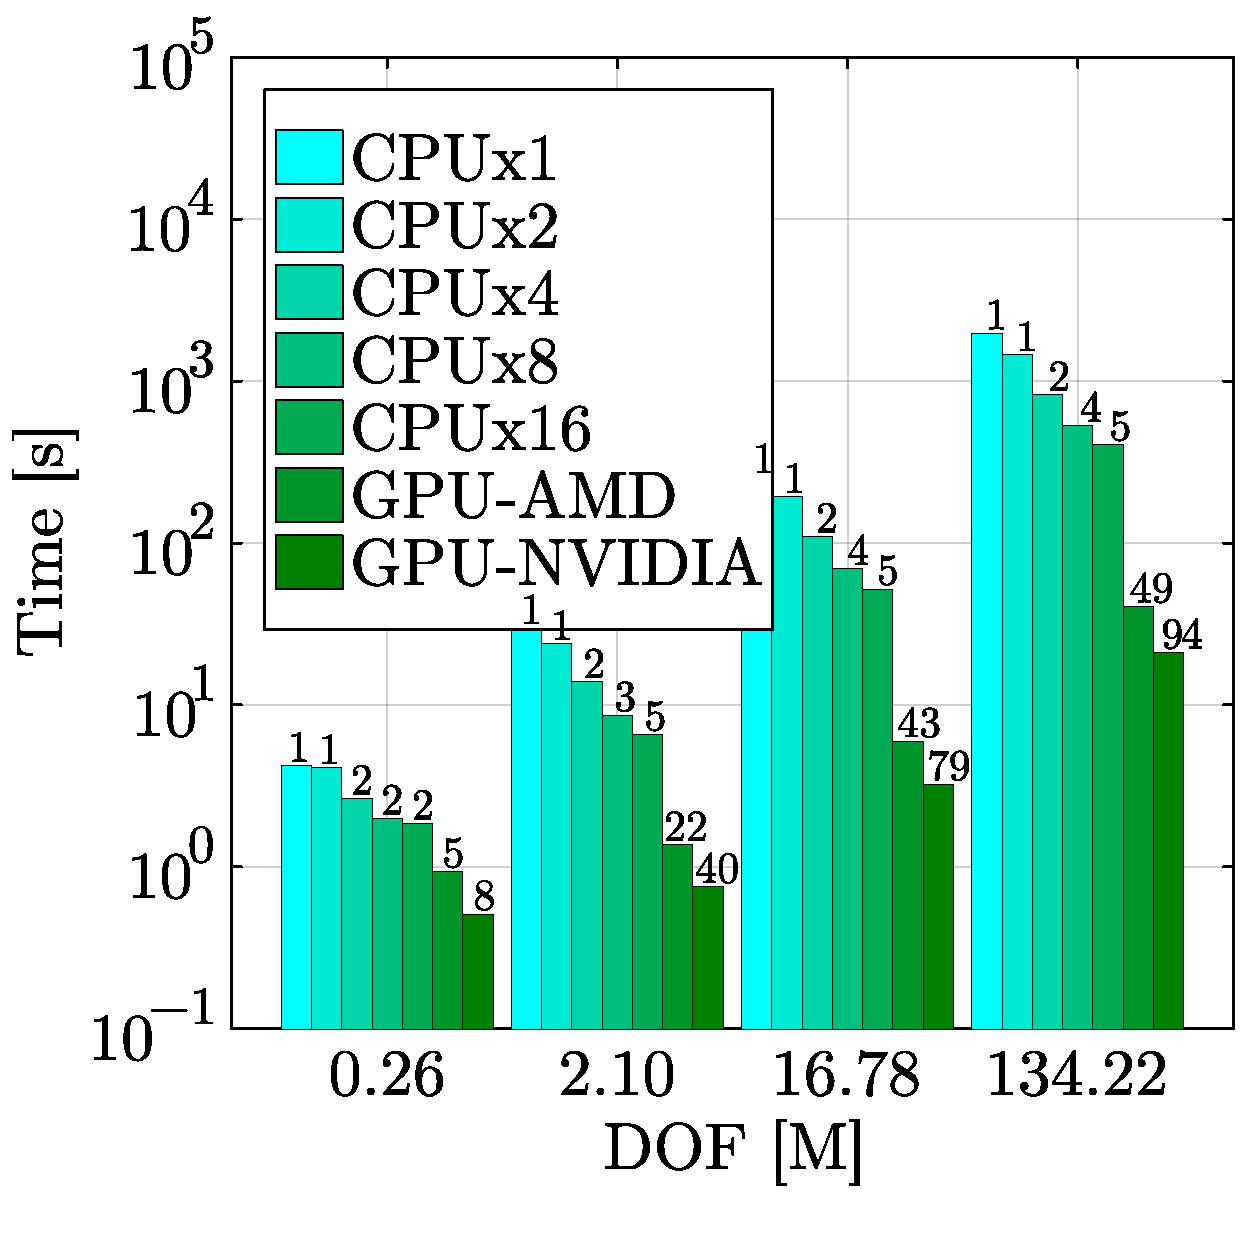
\includegraphics[width=\linewidth]{img/tgv_benchmark.pdf}
      \caption{TGV}
  \end{subfigure}
  \begin{subfigure}[t]{0.33\linewidth}
    \centering\hspace*{-0.2cm}
    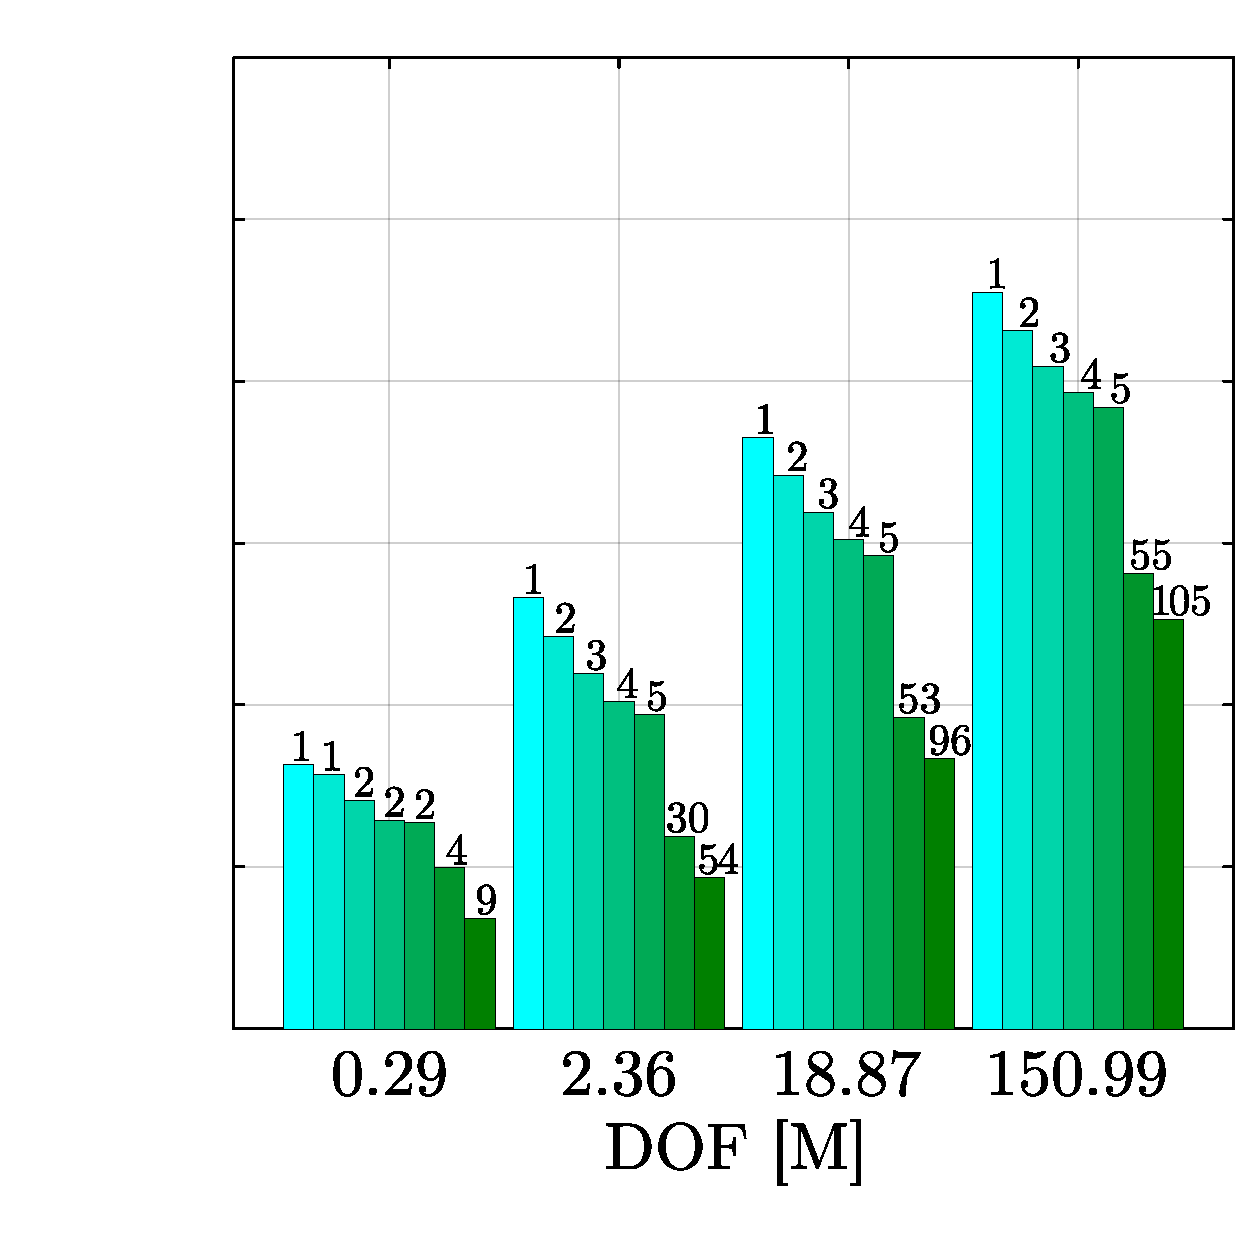
\includegraphics[width=\linewidth]{img/sphere_benchmark.pdf}
    \caption{Sphere}
  \end{subfigure}
  \begin{subfigure}[t]{0.33\linewidth}
    \centering\hspace*{-0.2cm}
    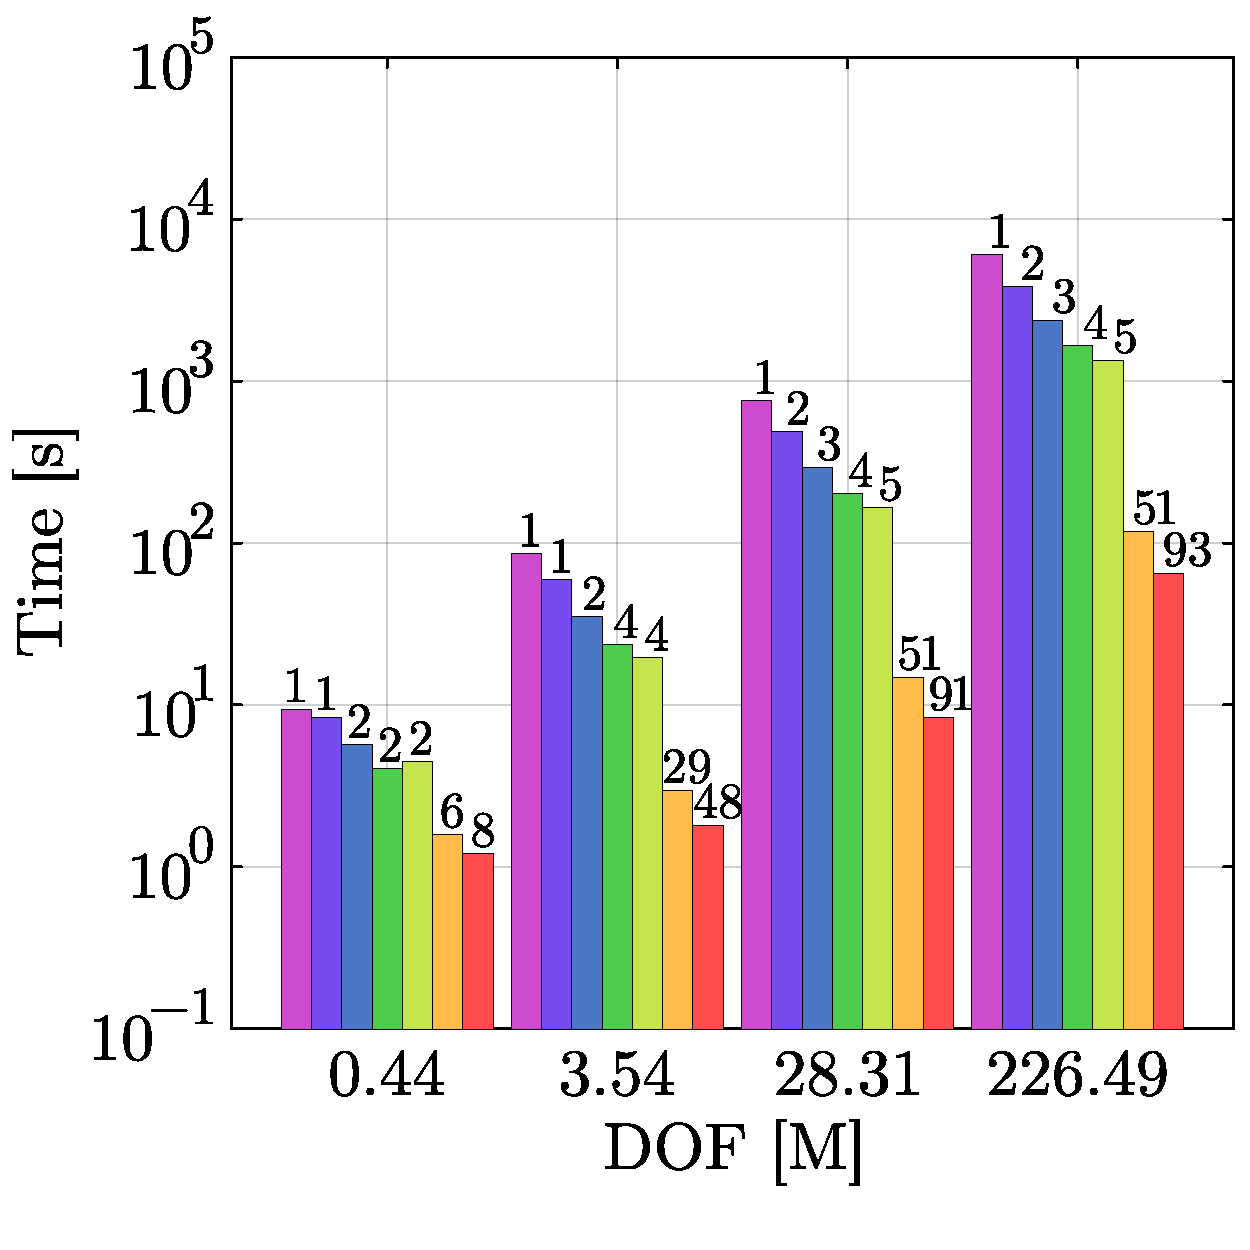
\includegraphics[width=\linewidth]{img/cylinder_benchmark.pdf}
    \caption{Moving cylinder}
  \end{subfigure}
	\caption{Time to run 100 time steps in single precision for the Taylor--Green vortex (left), fixed sphere (center), and moving cylinder (right) cases at different grid sizes. The CPU execution comprises multiple number of threads from single thread (serial) to 16 threads (multi-threading). The speedup for each case with respect to the serial execution (CPUx1) is shown above each bar. The speedup is computed as time(CPUx1)/time(X). The benchmarks have been run on an accelerated node of the Marenostrum5 supercomputer using Intel Xeon Platinum 8460Y @ 2.3GHz cores and a NVIDIA Hopper H100 64GB HBM2 GPU.}
	\label{fig:benchmarks}
\end{figure}

\begin{figure}[!ht]
  \centering
  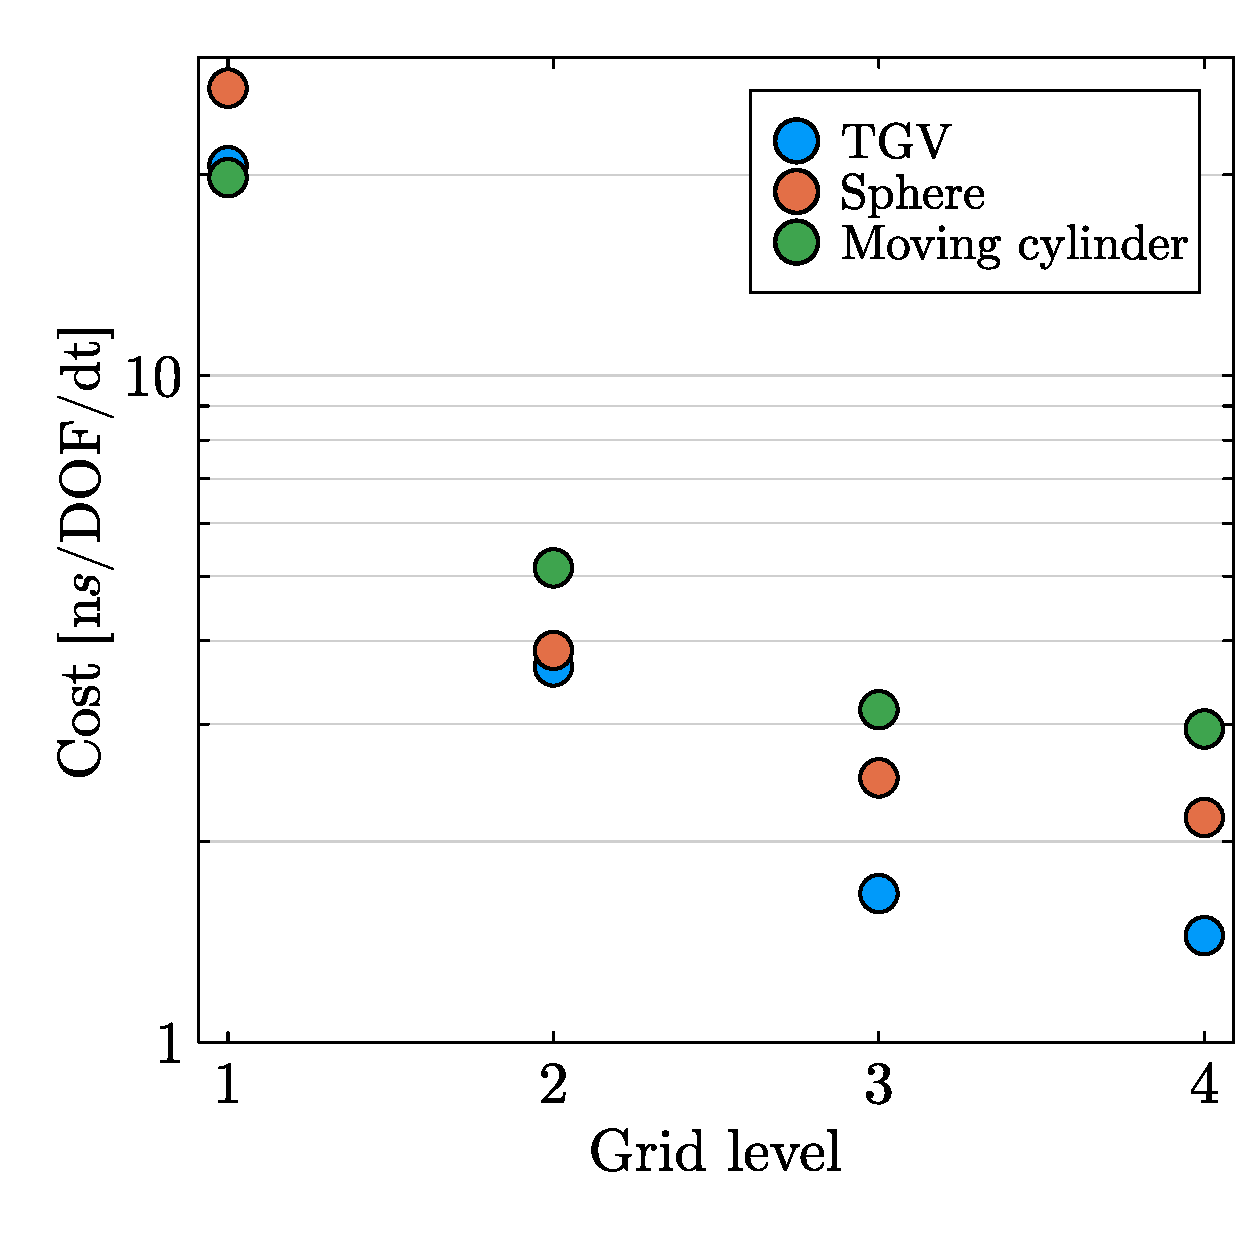
\includegraphics[width=0.4\linewidth]{img/cost.pdf}
\caption{Cost defined as execution time per grid DOF and time step on the different cases and grid levels. Data resulting from figure \ref{fig:benchmarks} benchmarks.}
\label{fig:cost}
\end{figure}

\begin{figure}[!ht]
  \centering
  \begin{subfigure}[t]{0.33\linewidth}
      \centering
      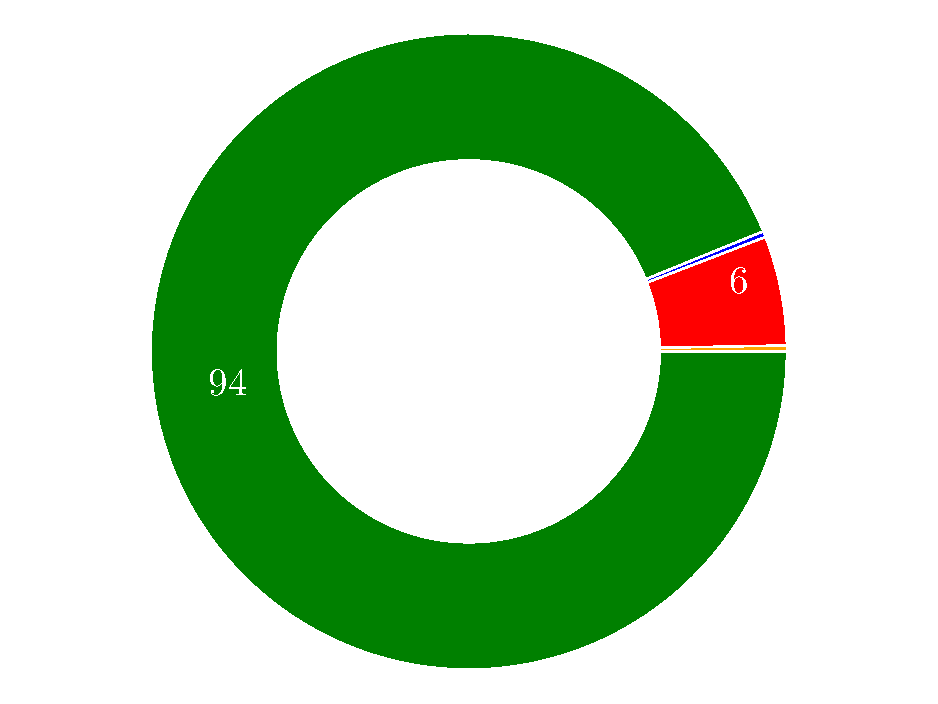
\includegraphics[width=\linewidth]{img/tgv_profile.pdf}
      \caption{TGV}
  \end{subfigure}
  \begin{subfigure}[t]{0.33\linewidth}
    \centering
    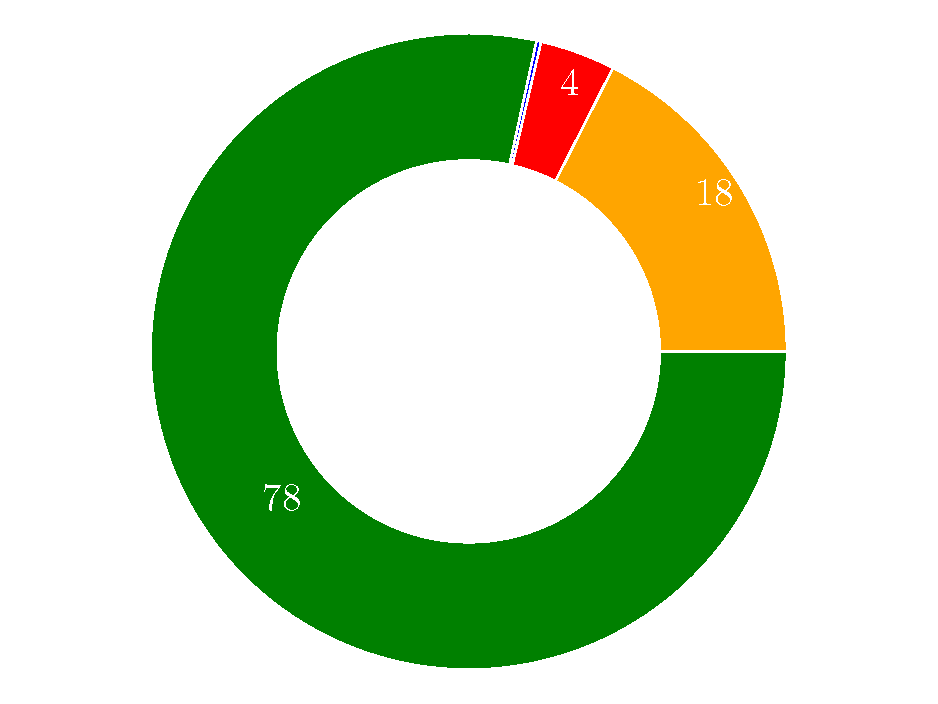
\includegraphics[width=\linewidth]{img/sphere_profile.pdf}
    \caption{Sphere}
  \end{subfigure}
  \begin{subfigure}[t]{0.33\linewidth}
    \centering
    \subcaptionbox{Moving cylinder\hspace*{5em}}{%
      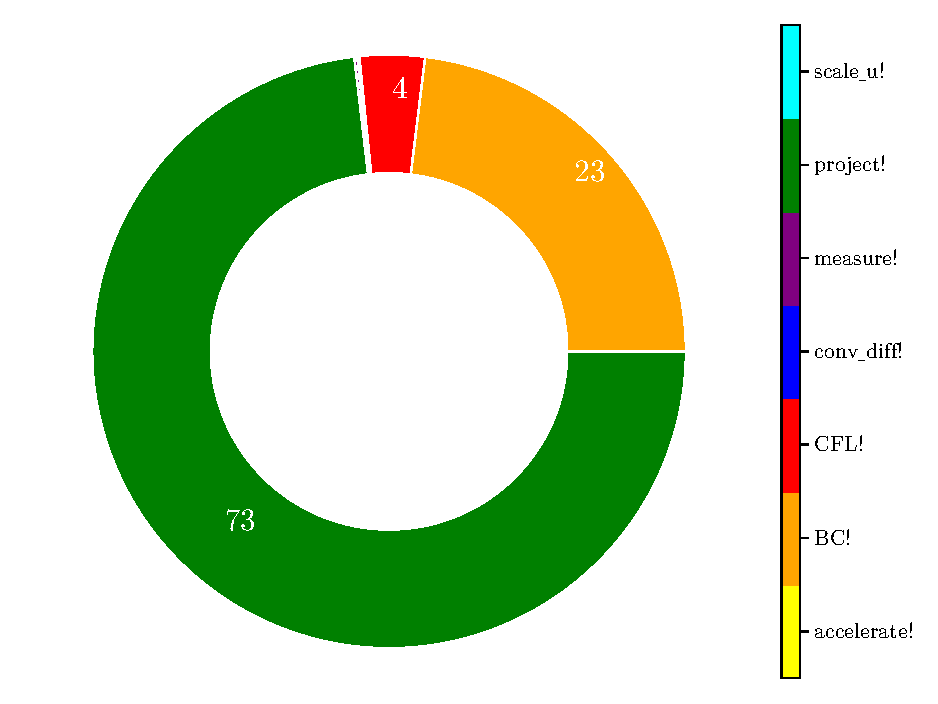
\includegraphics[width=\linewidth]{img/cylinder_profile.pdf}%
    }
  \end{subfigure}
  \caption{Kernel timings distribution for the 3rd-level grids of the different test cases. Timings are measured as the median value of the kernel execution time for 1000 time steps, noting that each kernel can be called more than once for each time step (ie. predictor-corrector scheme). We note that field ``BC!" accounts for all the following the boundary-conditions subroutines: ``BC!", ``BDIM!", ``BCTuple", ``exitBC!", where the latter is the most expensive one. Tests are conducted using single precision in an NVIDIA GeForce RTX 4060 Laptop GPU. During the tests, 99.9\% of time is spent in kernel execution while only 0.1\% is spent on device-to-host memory-copy calls (related to the pressure solver).}
\label{fig:profiling}
\end{figure}

\begin{figure}[!ht]
    \centering
    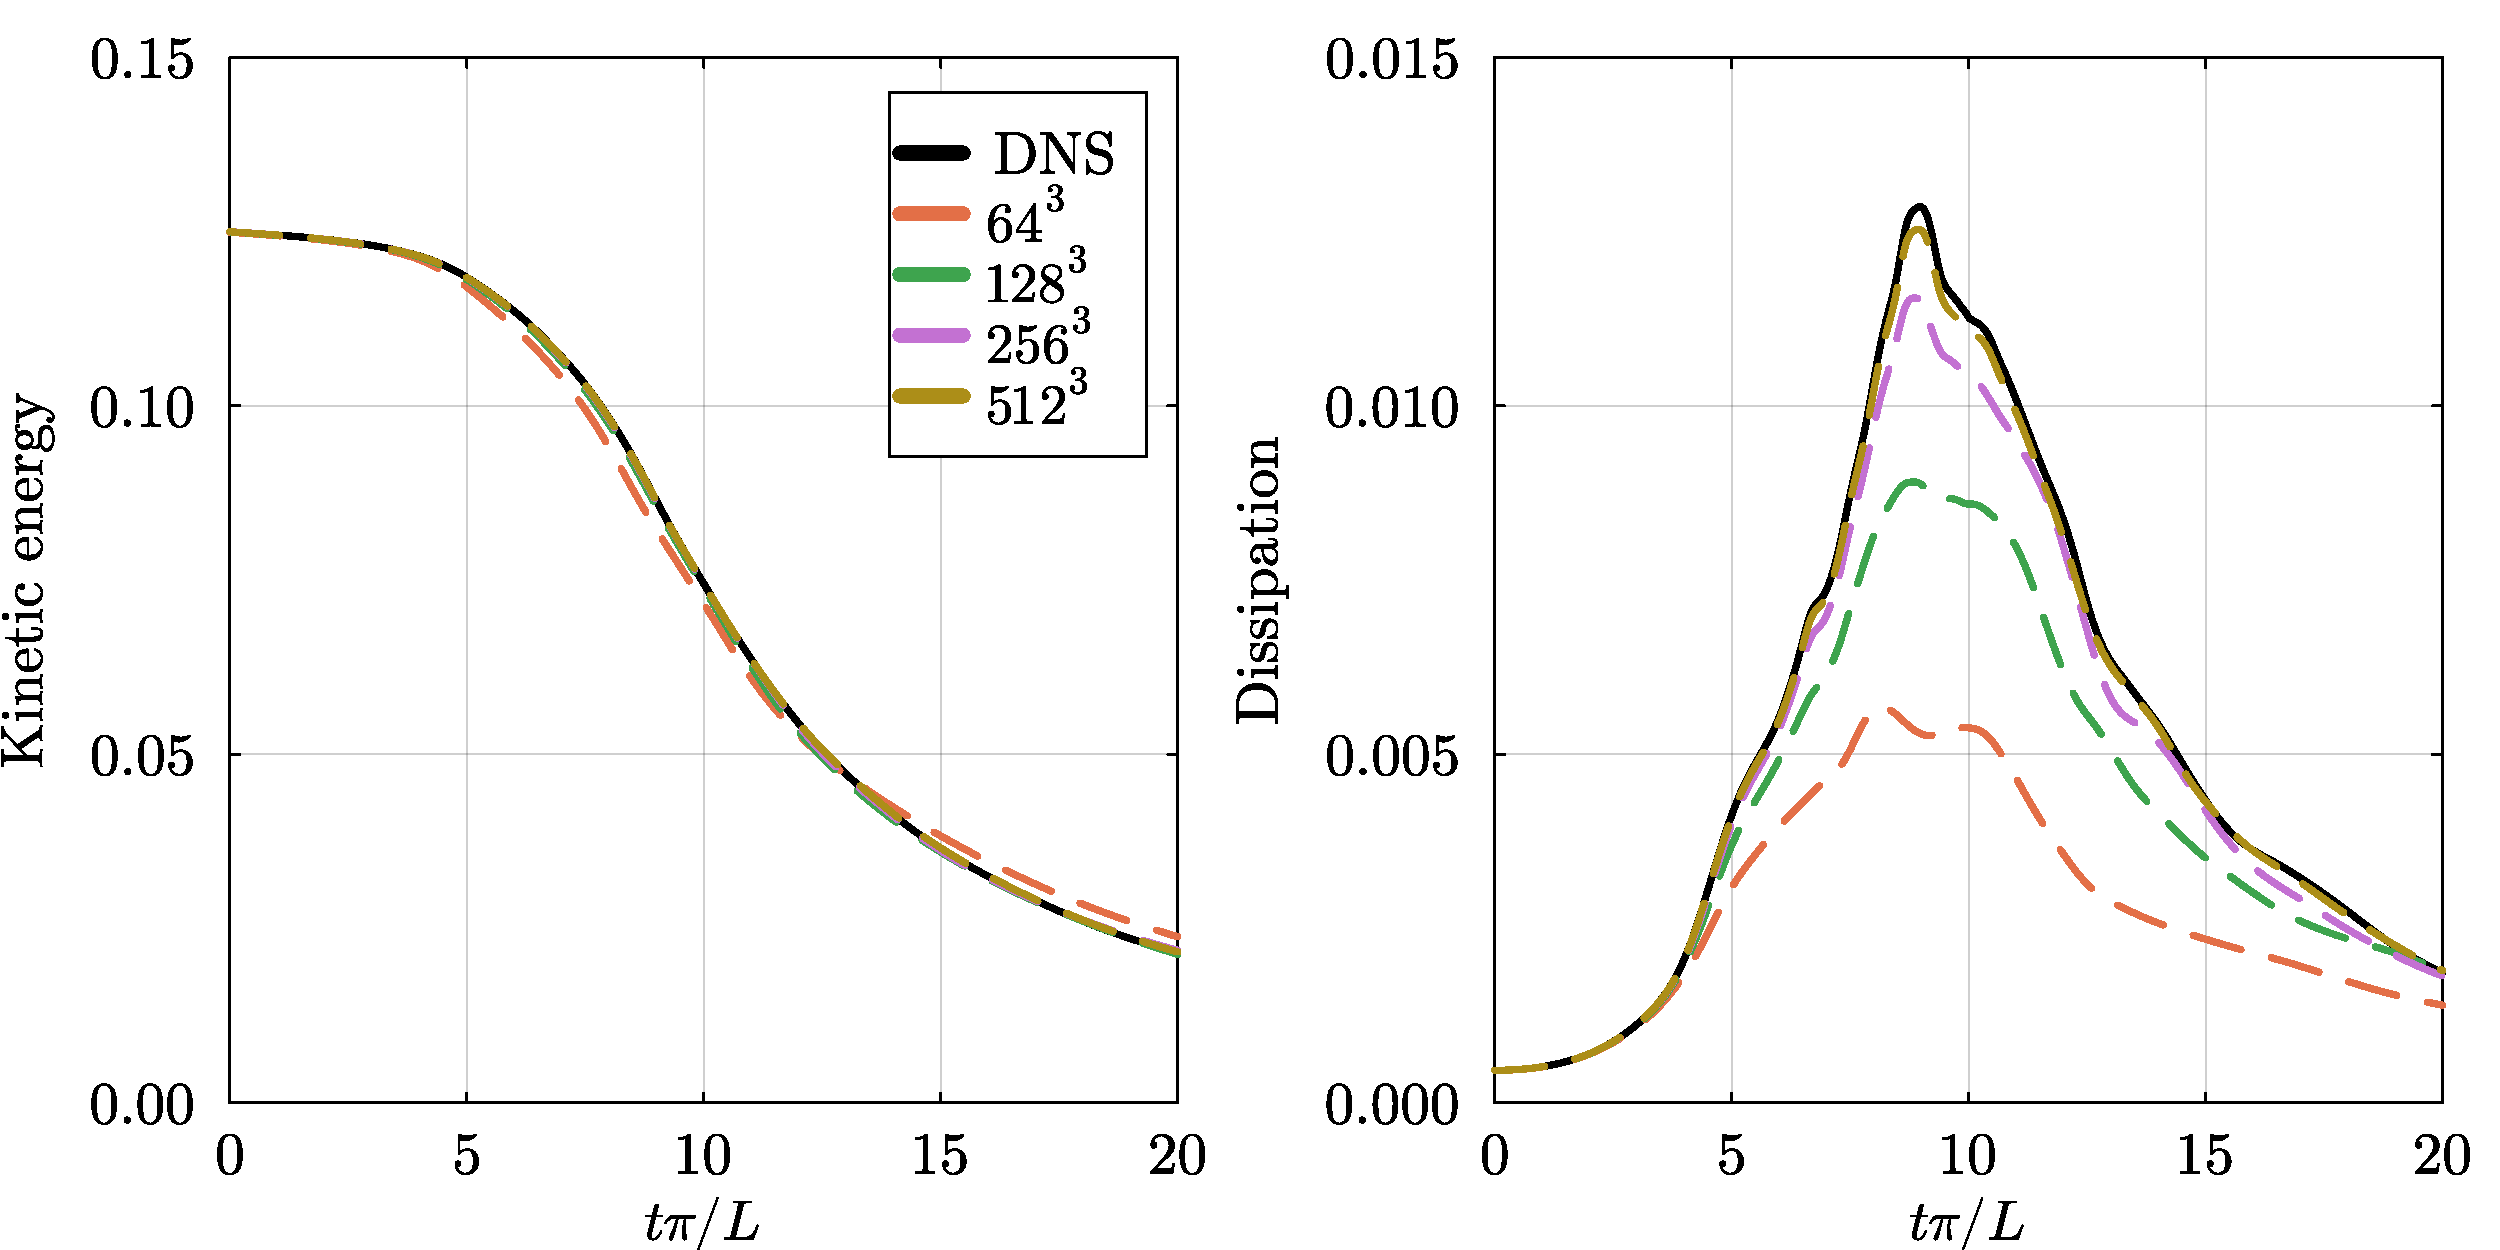
\includegraphics[width=0.8\linewidth]{img/tgv.pdf}
	\caption{Taylor--Green vortex (TGV) validation. Direct numerical simulation (DNS) data from \cite{Dairay2017} is used as reference.}
	\label{fig:tgv}
\end{figure}

\section{Sample applications}\label{sec:applications}
Three applications are selected to demonstrate the capability of the package to analyse general fluid flows. The examples also showcase the advantages of a differentiable back-end agnostic Cartesian-grid solver.

\subsection{Optimized control cylinders}

\begin{figure}
    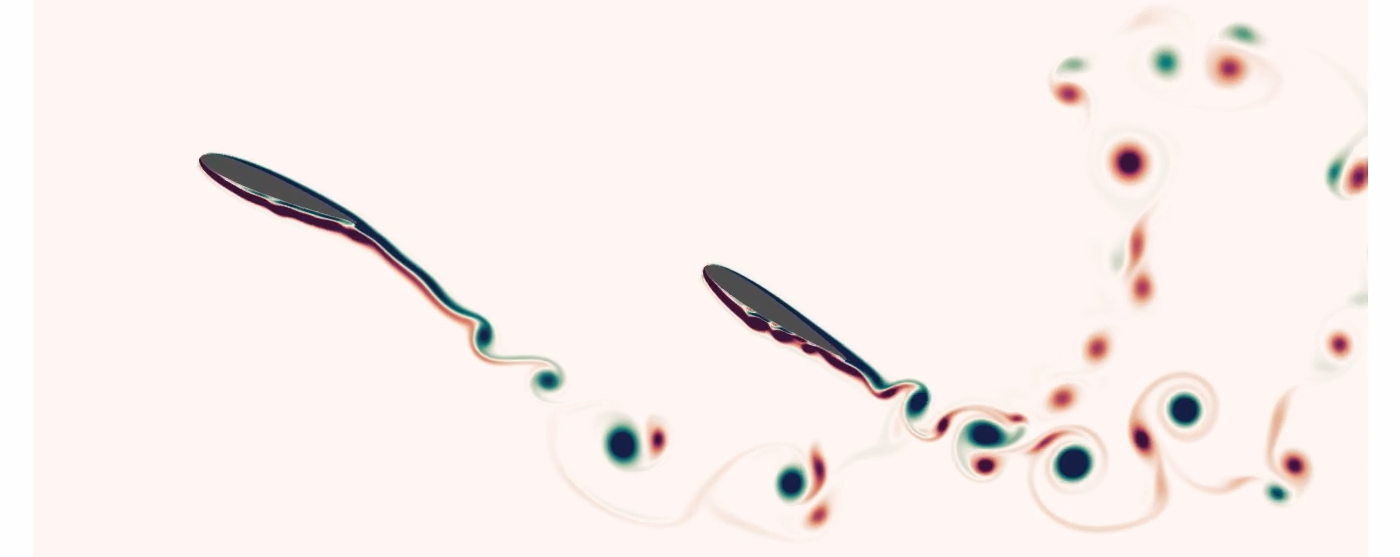
\includegraphics[width=\linewidth]{img/tandem.png}
    \caption{Tandem flapping foils}
    \label{fig:spinning_circle}
\end{figure}

The first example will be optimizing the controlled 2D flow around a circle using a pair of small spinning circles placed 120 degrees relative to the inflow direction, Fig~\ref{fig:spinning_circle}a. Experimental and numerical studies of this system have show the capability of the spinning cylinders to control the flow over the large circle [ref,ref], establishing a steady symmetric wake, reducing the system drag and even producing a net thrust as the rotation rate is increased.

The system is described by a few dimensionless ratios: $Re=UD/\nu$ the Reynolds number based on the large circle diameter and inflow velocity, as well as $d/D$, $g/D$ and $\xi=c/U$ the scaled diameter of the control circle, it's gap from the large circle surface, and it's scaled surface speed. This system is simulated with WaterLily using the values of $Re=500,\ d/D=0.15,\ g/D=0.05$ with grid resolution $D/h=96$. The domain is sized to $(6D,2D)$ taking advantage of the known symmetry of the flow by using a symmetry plane and only modelling the upper half of the full domain. WaterLily can combine AutoBodies based on the arithmetic of signed-distance functions, allowing the two bodies to be added to the simulation trivially.

We use the differentiable solver to maximize the scaled propulsive power $C_P = FU/\rho dc^3$ where $F$ is the net thrust force on the system. This metric is  proportional to the propulsive efficiency since $\rho dc^3$ scales with the power required to rotate the control cylinders [ref]. The time history of $C_P$ is plotted for a few values of $\xi$ in Fig~\ref{fig:spinning_circle}b, demonstrating that only a few convective cycles are required to reach steady state, as well as the control authority of $\xi$ over the propulsive power.

We optimize $\hat\xi=\text{argmin}\ C_P(\xi)$ at time $t^*=tU/L=2$ using Davidson's method [ref], which evaluates $C_P$ and it's derivative $\partial C_P/\partial \xi$ at points bracketing an optimum, using inverse cubic interpolation to iteratively restrict the interval. Both the value and derivative of the power are computed simultaneously using dual numbers, at a cost only 80\% larger than evaluating the function alone. Fig~\ref{fig:spinning_circle}c shows the resulting evaluation history starting with the interval $\xi=[3,8]$, leading to the optimum $\hat\xi\approx 6.25$ in a few iterations. Rates above this optimum produce more net thrust, but require excessive rotation rates to produce.

\subsection{Deforming and dynamic geometries}

The final two examples showcase the solvers ability to handle more complex geometries with ease. The first is a pulsing jellyfish-inspired geometry, and the second is a flapping butterfly-inspired geometry. Both of these cases are fast enough to simulate on a laptop GPU for live demonstrations.

The bell of the jellyfish is constructed with more AutoBody-arithmetic, in this case taking the difference of a hollow sphere with an oriented plane. This geometry is made to pulse by mapping the coordinates harmonically in the radial and transverse directions. While the geometry maintains a roughly constant solid volume throughout the pulse, small deviations are handled gracefully by the solver. Fig~\ref{} shows equally spaced snapshots of the geometry and resulting flow throughout the cycle. Each cycle generates a strong propulsive vortex ring which breaks up as it propagates away, in qualitative agreement with experimental studies [ref].

The butterfly geometry is a pair of membrane wings defined using the ParametricBodies package [ref]. The wing's planform is defined by a set of planar points which are interpolated using a cubic spline. The 3D distance function and normal to this planar membrane are then evaluated using a parametric root-finding method to immerse the geometry in the simulation as with the examples above. Harmonic coordinate rotations about the "shoulder" are used to flap the wings. Fig~\ref{} shows equally spaced snapshots of the geometry and resulting flow throughout the cycle. The classic clap-and-fling vortex formations are observed [ref].

\section{Conclusions}\label{sec:conclusions}

\section{Acknowledgements}\label{sec:acknowledgements}
\begin{itemize}
    \item BSC HPC services
    \item Dr. Lucas Gasparino
\end{itemize}

\bibliographystyle{elsarticle-num}
\bibliography{main.bib}

\end{document}

%%
%% End of file